\documentclass[12pt,a4paper]{article}
\usepackage[T1]{fontenc}
\usepackage{newtxtext,newtxmath}
\usepackage[margin=25mm]{geometry}
\usepackage{float,etoolbox,setspace,booktabs,tabularx,longtable,array,enumitem,xcolor,listings,fancyhdr,titlesec,microtype,needspace}
\usepackage[hidelinks]{hyperref}
\usepackage{tikz}
\usetikzlibrary{arrows.meta,positioning}
\definecolor{ink}{HTML}{17324D}
\definecolor{codebg}{HTML}{F4F6F8}
\onehalfspacing
\raggedbottom
\emergencystretch=3em
\clubpenalty=10000
\widowpenalty=10000
\BeforeBeginEnvironment{lstlisting}{\par\noindent\begin{minipage}{\linewidth}}
\AtBeginEnvironment{lstlisting}{\singlespacing}
\AfterEndEnvironment{lstlisting}{\end{minipage}\par}
\AtBeginEnvironment{table}{\singlespacing}
\AtBeginEnvironment{tabular}{\singlespacing}
\setlength{\parindent}{1.25cm}
\setlength{\parskip}{3pt}
\setlength{\headheight}{16pt}
\pagestyle{fancy}
\fancyhf{}
\fancyfoot[C]{\thepage}
\renewcommand{\headrulewidth}{0pt}
\titleformat{\section}{\large\bfseries\color{ink}}{\thesection.}{0.6em}{}
\titleformat{\subsection}{\normalsize\bfseries}{\thesubsection.}{0.6em}{}
\titlespacing*{\section}{0pt}{14pt}{8pt}
\titlespacing*{\subsection}{0pt}{10pt}{5pt}
\setlist{nosep,leftmargin=1.5em}
\lstset{language=Java,basicstyle=\ttfamily\footnotesize,keywordstyle=\bfseries\color{ink},commentstyle=\itshape\color{gray},stringstyle=\color{teal!70!black},backgroundcolor=\color{codebg},frame=single,rulecolor=\color{gray!30},breaklines=true,columns=fullflexible,keepspaces=true,showstringspaces=false,tabsize=4,aboveskip=8pt,belowskip=8pt,captionpos=b}
\newcommand{\code}[1]{\texttt{#1}}
\pretocmd{\section}{\Needspace{8\baselineskip}}{}{}
\pretocmd{\subsection}{\Needspace{5\baselineskip}}{}{}
\renewcommand{\arraystretch}{1.08}
\newcolumntype{Y}{>{\raggedright\arraybackslash}X}
\begin{document}
\section{Program Structure}
\subsection{Purpose and implementation scope}
The purpose of this laboratory work is to design a small logging library and use it to explain the execution of a parentheses-validation algorithm. The implementation demonstrates encapsulation, the distinction between class-level and object-level state, method delegation, enumeration types, and collaboration between objects. The logger is implemented directly rather than obtained from an external framework, because its behavior is the subject of the exercise.

The program supports the four required levels, a configurable minimum severity, and the placeholders \code{\%t}, \code{\%m}, \code{\%n}, and \code{\%l}. It also implements the optional \code{\%r} placeholder. The validation result is returned as Java's primitive \code{boolean}; log messages describe the execution but do not determine that result.

\subsection{Responsibilities of the program types}
\begin{table}[H]
\centering\small
\begin{tabularx}{\textwidth}{@{}p{0.33\textwidth}Y@{}}
\toprule
\textbf{Type / source file} & \textbf{Responsibility in this implementation}\\
\midrule
\code{LogLevel.java} & Defines the finite severity set, stores explicit severity values and per-level phrases, compares levels, and selects a random phrase.\\
\code{Logger.java} & Stores a logger name; manages shared configuration; checks message severity; substitutes placeholders; writes accepted messages to the console.\\
\code{ParenthesesValidator.java} & Checks ordering and matching of round parentheses, returns validity, and reports events through its logger.\\
\code{Main.java} & Configures the application and demonstrates the four inputs required by the handout.\\
\bottomrule
\end{tabularx}
\caption{Responsibilities of the four implementation types.}
\end{table}

The responsibility of \code{Logger} is presentation and filtering of diagnostic information. The responsibility of \code{ParenthesesValidator} is the correctness decision about the input. Keeping these responsibilities separate allows the format or severity threshold to change without changing the counter-based algorithm.

\subsection{Collaboration and direction of dependency}
\begin{center}
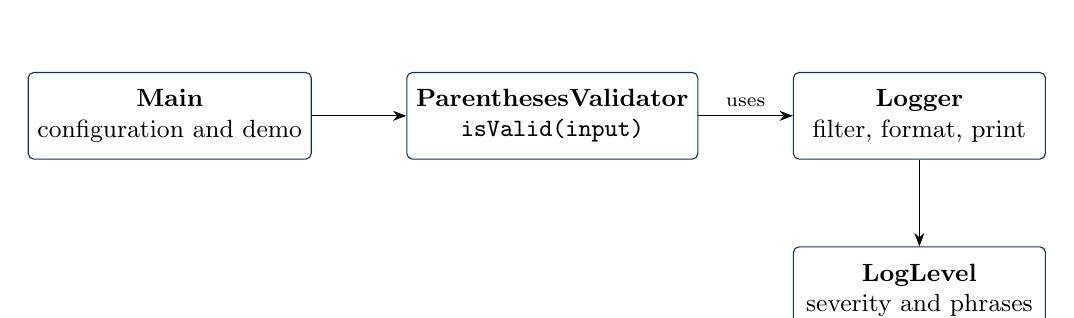
\begin{tikzpicture}[node distance=11mm and 12mm,box/.style={draw=ink,rounded corners=2pt,align=center,minimum width=32mm,minimum height=11mm,font=\small},>=Stealth]
\node[box] (main) {\textbf{Main}\\configuration and demo};
\node[box,right=of main] (validator) {\textbf{ParenthesesValidator}\\\code{isValid(input)}};
\node[box,right=of validator] (logger) {\textbf{Logger}\\filter, format, print};
\node[box,below=of logger] (level) {\textbf{LogLevel}\\severity and phrases};
\draw[->] (main) -- (validator);
\draw[->] (validator) -- node[above,font=\scriptsize]{uses} (logger);
\draw[->] (logger) -- (level);
\end{tikzpicture}
\end{center}
The validator contains a reference to a \code{Logger} named \code{Parentheses}. This is object composition: the validator has a logger and delegates diagnostic work to it. The validator does not extend \code{Logger}; a validator is not a specialized kind of logger. The logger does not depend on the parentheses problem and can therefore be reused elsewhere.

\section{Classes and Objects}
\subsection{A class and an object in the program}
A class describes the fields and methods of a type. In this implementation, \code{Logger} specifies that each logger has a name and can process messages through \code{log()}, \code{trace()}, \code{info()}, \code{warn()}, and \code{error()}. An object is a particular instance created from that class.

\begin{samepage}
The following declarations appear in the implementation:
\begin{lstlisting}
// Main.java: create the validator used by the demonstration.
ParenthesesValidator validator = new ParenthesesValidator();

// ParenthesesValidator.java: create its diagnostic collaborator.
private final Logger logger = new Logger("Parentheses");
\end{lstlisting}
\end{samepage}
The local variable \code{validator} stores a reference to a validator object. Constructing that object initializes its \code{logger} field with a reference to a distinct logger object. Calling \code{isValid()} executes a method on the validator. Calls to \code{logger.trace(...)} execute methods on the logger collaborator.

\subsection{State stored by each object}
A logger instance stores its own \code{name} reference. The field is private, so outside code cannot assign to it directly, and final, so the constructor assigns it only once. The associated \code{String} is immutable. Creating another logger with another name does not change the first logger's name.

A validator instance stores its \code{logger} reference. It does not store the current input or balance as fields. The parameter \code{input} and local variables \code{balance}, \code{i}, and \code{current} exist for a particular method invocation. This distinction matters: a second validation call starts with a new local balance of zero rather than reusing the previous call's count.

\code{Main} is used as an entry-point class. Its static \code{main()} method creates the demonstration objects; it does not require a \code{new Main()} instance. The input array belongs to that method invocation rather than to the class as a static field.

\subsection{Why the levels are an enum rather than a record}
\code{LogLevel} is an enum because the specification defines a closed set of four values: \code{TRACE}, \code{INFO}, \code{WARN}, and \code{ERROR}. Each constant is an instance of the enum type and has its own severity and phrase array. For example, \code{TRACE} has severity 10, while \code{ERROR} has severity 40.

A record would be useful for a data aggregate, such as a future log entry containing a timestamp, level, name, and message. It is unnecessary for the fixed severity set: a general record constructor would permit additional name/severity combinations unless extra restrictions were introduced. The enum already provides the required finite vocabulary and a natural place for level-specific metadata.

The fields \code{severity} and \code{phrases} are final. For the array, final prevents replacing the array reference; it does not make array elements immutable. The current implementation does not expose the array, and \code{randomPhrase()} returns only a selected \code{String}. Thus callers do not receive a mutable reference to the stored phrase collection.

\section{Static and Instance Members}
\subsection{Shared configuration and individual identity}
The required logger configuration is class-level state. There is one \code{level} field and one \code{format} field for the loaded \code{Logger} class, shared by its instances. The name, by contrast, belongs to each particular logger.

\begin{samepage}
\begin{lstlisting}
private final String name;

private static LogLevel level = LogLevel.INFO;
private static String format = "[%t] [%l] %n: %m";

private static final DateTimeFormatter TIME_FORMAT =
        DateTimeFormatter.ofPattern("HH:mm:ss");
\end{lstlisting}
\end{samepage}

\begin{table}[H]
\centering\small
\begin{tabularx}{\textwidth}{@{}p{0.22\textwidth}p{0.23\textwidth}Y@{}}
\toprule
\textbf{Member} & \textbf{Kind} & \textbf{Reason and effect}\\
\midrule
\code{name} & Instance, final & Identifies one logger and is fixed after construction.\\
\code{level} & Static, mutable & Applies one minimum severity to all logger instances.\\
\code{format} & Static, mutable & Applies one output template to all logger instances.\\
\code{TIME\_FORMAT} & Static, final & Reuses one immutable time formatter for all loggers.\\
\code{setLevel()} & Static method & Updates class-level severity configuration.\\
\code{setFormat()} & Static method & Updates class-level formatting configuration.\\
\code{log()} & Instance method & Uses the receiving logger's individual name.\\
\bottomrule
\end{tabularx}
\caption{Class-level and object-level members of \code{Logger}.}
\end{table}

\begin{samepage}
\begin{samepage}
\subsection{What happens when the level changes?}
The setter assigns the shared field after rejecting a null argument:
\begin{lstlisting}
public static void setLevel(LogLevel newLevel) {
    level = Objects.requireNonNull(
            newLevel, "Log level cannot be null");
}
\end{lstlisting}
\end{samepage}
Consequently, changing the level affects both existing and subsequently created loggers. The following explanatory example illustrates that behavior; it is not an additional source file in the submitted program.
\begin{lstlisting}
Logger first = new Logger("First");
Logger second = new Logger("Second");

Logger.setLevel(LogLevel.ERROR);
first.info("Hidden");
second.warn("Hidden");
first.error("Visible");
second.error("Also visible");
\end{lstlisting}
\end{samepage}
The names remain \code{First} and \code{Second}, but both loggers consult the same updated minimum severity. Making \code{level} an ordinary instance field would instead permit different thresholds per object and would not implement the handout's required shared configuration.

The same reasoning applies to \code{setFormat()}. Static does not mean constant: \code{level} and \code{format} are deliberately mutable. The distinct \code{static final} declaration of \code{TIME\_FORMAT} indicates a shared reference that is not reassigned. These are separate design decisions.

\section{Methods and Responsibilities}
\subsection{The processing pipeline in \code{log()}}
The public \code{log()} method is the common entry point for logging behavior. It checks its arguments, applies severity filtering, formats accepted messages, and prints the resulting line. It does not validate parentheses or decide whether a program input is correct.

\begin{samepage}
\begin{lstlisting}
public void log(LogLevel messageLevel, String message) {
    Objects.requireNonNull(messageLevel,
            "Message level cannot be null");
    Objects.requireNonNull(message,
            "Message cannot be null");

    if (!level.allows(messageLevel)) {
        return;
    }

    System.out.println(formatMessage(messageLevel, message));
}
\end{lstlisting}
\end{samepage}

An argument error is handled differently from an invalid parentheses string. Passing a null level or message to the logger is a misuse of its API and produces a \code{NullPointerException} through \code{Objects.requireNonNull()}. Passing a null string to the validator is treated as invalid input and returns false after logging a reason. Concatenating that input into the diagnostic message produces the text \code{null}, not a null message reference.

Filtering precedes formatting. A hidden message is not formatted or printed, and its random phrase is not selected. However, ordinary Java argument evaluation still happens before the method is called: a message constructed by string concatenation in the validator has already been built. This logger does not implement lazy message suppliers.

\begin{samepage}
\subsection{Level comparison and the filtering matrix}
The enum compares explicit severity values rather than declaration positions:
\begin{lstlisting}
public boolean allows(LogLevel messageLevel) {
    return messageLevel.severity >= this.severity;
}
\end{lstlisting}
\end{samepage}
Here, \code{this} is the configured threshold and \code{messageLevel} describes the current entry. A message of exactly the configured severity is accepted because the comparison includes equality.

\begin{center}\small
\begin{tabular}{@{}lcccc@{}}
\toprule
\textbf{Configured minimum} & \textbf{TRACE} & \textbf{INFO} & \textbf{WARN} & \textbf{ERROR}\\
\midrule
TRACE & Print & Print & Print & Print\\
INFO & Hide & Print & Print & Print\\
WARN & Hide & Hide & Print & Print\\
ERROR & Hide & Hide & Hide & Print\\
\bottomrule
\end{tabular}
\end{center}
Using numeric values 10, 20, 30, and 40 makes the severity relationship explicit. The numbers are not output labels; the enum names are used when replacing \code{\%l}.

\subsection{Convenience methods and delegation}
\code{trace()}, \code{info()}, \code{warn()}, and \code{error()} delegate to \code{log()} with a fixed level. For example, \code{info(message)} calls \code{log(LogLevel.INFO, message)}. This avoids duplicating argument checks, filtering, and formatting in four methods. It also makes validator code readable: \code{logger.info("Matching pair completed at index " + i)} states the event severity directly.

\subsection{Configurable formatting}
The private \code{formatMessage()} method converts the template into a concrete output line. It copies the configured format into a local variable, obtains the current local time once, and accumulates output using \code{StringBuilder}. Its supported tokens are summarized below.

\begin{table}[H]
\centering\small
\begin{tabularx}{\textwidth}{@{}lY@{}}
\toprule
\textbf{Token} & \textbf{Replacement in this implementation}\\
\midrule
\code{\%t} & Local time obtained for this entry, formatted as \code{HH:mm:ss}.\\
\code{\%l} & Name of the current message's enum level.\\
\code{\%n} & Name of the logger object receiving the call.\\
\code{\%m} & The original message string, inserted literally.\\
\code{\%r} & One random phrase associated with the current message level.\\
\bottomrule
\end{tabularx}
\caption{Required placeholders and the extra-credit placeholder.}
\end{table}

The scanner processes the template from left to right. A normal character is appended directly. A percent sign with a following character is examined by a \code{switch}; recognized tokens append their values, while an unknown token appends both original characters. After processing a two-character token, the extra \code{i++} skips its second character. A percent sign at the end is appended directly because there is no following token character.

\begin{samepage}
\begin{lstlisting}
char current = template.charAt(i);

if (current != '%' || i + 1 >= template.length()) {
    result.append(current);
    continue;
}

char placeholder = template.charAt(i + 1);
\end{lstlisting}
\end{samepage}

For example, the format \code{[\%l] \%n: \%m} can produce \code{[INFO] Parentheses: Valid input}. A format containing only \code{\%m} produces only the message. A repeated token such as \code{\%l / \%l} is replaced at both positions. Unknown \code{\%x} and an isolated trailing percent sign remain literal.

The formatter scans the template, not the text that it inserts. Therefore, if a message itself contains \code{\%l}, that text remains unchanged. This avoids recursive substitution and the order-dependent behavior that can occur with a sequence of global replacements. There is no separately specified escaping syntax for arbitrary runs of percent signs; the implemented scanner defines their processing.

Time is captured once per accepted entry, so repeated \code{\%t} tokens in that entry agree. In the present code, time is obtained even when the template omits \code{\%t}; this is a small potential optimization, not a correctness issue. The local template reference gives one entry a stable format snapshot, but it does not make the entire logger thread-safe.

\subsection{Why logging is delegated by the validator}
The validator knows when an opening parenthesis, matching pair, or invalid condition occurs. It reports those semantic events and leaves their representation to the logger. If it implemented formatting and filtering itself, every validation branch would need to manage those details. Delegation centralizes that behavior and keeps the validation decision independent of the chosen display settings.

\subsection{Extra credit: level-specific random phrases}
Each enum constant is constructed with a severity and three phrases. The constructor uses a varargs parameter, \code{String... phrases}, which is represented as an array inside the constructor. The random selection method is:

\begin{samepage}
\begin{lstlisting}
public String randomPhrase() {
    int index = ThreadLocalRandom.current()
            .nextInt(phrases.length);
    return phrases[index];
}
\end{lstlisting}
\end{samepage}

The upper bound is exclusive, so an array with three phrases uses valid indexes 0, 1, or 2. Selection is from the message's own enum constant: an \code{ERROR} entry uses \code{ERROR} phrases even when the configured minimum is \code{TRACE}. The threshold controls visibility; it does not classify the entry.

\begin{samepage}
\begin{lstlisting}
case 'r':
    if (randomPhrase == null) {
        randomPhrase = messageLevel.randomPhrase();
    }
    result.append(randomPhrase);
    break;
\end{lstlisting}
\end{samepage}

The local variable begins as null and is populated only when the first \code{\%r} token is encountered. Additional occurrences reuse the selected phrase for consistency within that line. Different entries can select different phrases, but consecutive selections may also repeat; randomness does not imply guaranteed alternation.

The selected phrase supplements the actual diagnostic message. A short generic phrase accompanies the specific reason describing an unmatched closing parenthesis and its index. That specific reason remains available through \code{\%m}, which carries the information needed to understand the failure.

\subsection{Event mapping and the invalid-result helper}
The validator uses \code{TRACE} after increasing the opening-parenthesis count, and \code{INFO} after completing a pair. It uses the optional \code{WARN} when a closing parenthesis has no available opening. Every invalid branch calls one helper:

\begin{samepage}
\begin{lstlisting}
private boolean reportInvalid(String input, String reason) {
    logger.error("Invalid input \"" + input + "\": " + reason);
    logger.info("Validation result for \"" + input + "\": false");
    return false;
}
\end{lstlisting}
\end{samepage}

Centralizing this path ensures that early returns still produce an error explanation and the final informational result. The valid path logs its final true result after the scan. At an \code{ERROR} threshold, the informational result call still occurs but its output is hidden; the helper still returns false. Thus console visibility and the returned result remain separate concerns.

\section{Testing and Correctness}
\subsection{Build environment and verification scope}
The inspected implementation contains four Java source files and no automated test suite. The demonstration was compiled with the available JDK 21 environment and run from a separate build directory during report preparation. The four required cases were observed in the resulting console output. No test files or application-source changes were added for this report.

\begin{samepage}
To compile and run the program from the laboratory directory:
\begin{lstlisting}[language={},basicstyle=\ttfamily\small]
javac -d out src/*.java
java -cp out Main
\end{lstlisting}
\end{samepage}
The first command compiles the source files into \code{out}; the second uses that directory as the classpath and launches \code{Main}. The current demonstration sets the threshold to \code{TRACE} and the format to \code{[\%l] \%n: \%m | \%r}, so all four event severities can appear. This explicit format overrides the logger's default and does not display the timestamp.

\subsection{Observed required examples}
\begin{table}[H]
\centering\small
\begin{tabularx}{\textwidth}{@{}p{0.25\textwidth}ccY@{}}
\toprule
\textbf{Input} & \textbf{Expected} & \textbf{Observed final log} & \textbf{Explanation}\\
\midrule
\code{()} & true & true & One opening is followed by its closing parenthesis.\\
\code{)((()))} & false & false & The first character is an unmatched closing parenthesis.\\
\code{(} & false & false & One opening remains unmatched at the end.\\
\code{(())((()())())} & true & true & Every prefix has enough openings, and the final balance is zero.\\
\bottomrule
\end{tabularx}
\caption{Results observed when running the supplied \code{Main} demonstration.}
\end{table}

These results were observed through the final \code{INFO} messages. The current \code{Main} calls \code{isValid()} but discards the returned boolean; it contains no assertions. The source confirms that the same branches return the corresponding true or false values. Accordingly, this table documents a manual demonstration, not an automated assertion-based test run.

For the valid input \code{()}, the log records an opening at index 0, a completed pair at index 1, and a final true result. For the invalid input \code{(}, it records the opening and then reports one unmatched opening together with a final false result. In each case, the random suffix may vary between runs without changing the decision.

\subsection{A check that prevents an ordering error}
The supplied \code{)((()))} case is particularly useful for checking the early-closing guard. The observed warning and error both identify index 0, demonstrating that a closing parenthesis is rejected when no opening is available. This protects the ordering requirement and avoids continuing with an invalid prefix. It does not establish that a particular historical bug occurred; it provides concrete evidence that the required guard is executed.

\subsection{How the algorithm establishes validity}
Let $b$ be the balance of unmatched openings in the processed prefix. Initially $b=0$. Reading \code{(} increases $b$ by one. Reading \code{)} is allowed only when $b>0$, after which $b$ decreases by one. Any other character is rejected under the implementation's chosen input policy.

A string over the two-character alphabet of round parentheses is valid exactly when both conditions hold:
\begin{enumerate}
\item Every prefix contains at least as many openings as closings.
\item The complete string contains equally many openings and closings.
\end{enumerate}
The early-closing guard enforces the first condition. The final \code{balance == 0} decision, implemented by rejecting a positive remaining balance and otherwise returning true, enforces the second. Both conditions are necessary: equal totals alone would incorrectly accept \code{)(}.

\begin{samepage}
\begin{lstlisting}
if (balance == 0) {
    // A closing parenthesis cannot be matched.
    return reportInvalid(input,
            "Unmatched closing parenthesis at index " + i);
}
balance--;
\end{lstlisting}
\end{samepage}
This excerpt shows the decision and omits the optional warning call for brevity. In the source, the warning is emitted before the invalid-result helper is called.

\subsection{Illustrative trace of a nested valid input}
The following trace is derived from the algorithm for \code{(())}; it is an explanatory walkthrough rather than an additional recorded execution of \code{Main}.

\begin{center}\small
\begin{tabular}{@{}ccccc@{}}
\toprule
\textbf{Index} & \textbf{Character} & \textbf{Balance before} & \textbf{Balance after} & \textbf{Event}\\
\midrule
0 & \code{(} & 0 & 1 & TRACE: opening found\\
1 & \code{(} & 1 & 2 & TRACE: opening found\\
2 & \code{)} & 2 & 1 & INFO: pair completed\\
3 & \code{)} & 1 & 0 & INFO: pair completed\\
\bottomrule
\end{tabular}
\end{center}
The counter is sufficient because all openings have the same type. The algorithm need not store their indexes to decide validity. Its matching-pair log identifies the closing index, but does not claim to identify the corresponding opening index. Supporting several bracket types or reporting exact opening/closing index pairs would require additional information, commonly a stack.

\subsection{Termination and repeated calls}
The loop advances its index through a finite string, or terminates earlier on an invalid character or unmatched closing parenthesis. A null argument is handled before accessing \code{input.length()}. At the end of a non-rejected scan, the balance cannot be negative. If it is positive, at least one opening is unmatched; if it is zero, all openings have been matched in a valid order.

Because \code{balance} is local, separate calls on the same validator do not share the counter. This prevents one incomplete input from contaminating the result of the next input, which is important because \code{Main} reuses one validator for all four examples.

\subsection{Boundary behavior and verification limits}
The following behaviors follow from source inspection. They are not claimed as additional executed tests in the repository.

\begin{table}[H]
\centering\small
\begin{tabularx}{\textwidth}{@{}p{0.20\textwidth}p{0.16\textwidth}Y@{}}
\toprule
\textbf{Input / situation} & \textbf{Result} & \textbf{Reason from the implementation}\\
\midrule
Empty string & true & No scan iterations occur; balance remains zero.\\
\code{null} & false & The explicit null guard calls \code{reportInvalid()}.\\
\code{)(} & false & The first closing parenthesis has no available opening.\\
\code{(()} & false & One opening remains after scanning.\\
\code{())} & false & The final closing parenthesis is unmatched.\\
\code{()()} & true & Both pairs close and the final balance is zero.\\
\code{(a)} & false & The non-parenthesis character is rejected.\\
\bottomrule
\end{tabularx}
\caption{Boundary behaviors established by reading the current source.}
\end{table}

The handout does not explicitly define null, empty-string, or unrelated-character policies. The program's choices are therefore documented as implementation decisions. In particular, it validates a string consisting exclusively of parentheses; it does not ignore ordinary characters inside an arbitrary expression.

The four-case demonstration does not exhaustively check every level/threshold combination, formatting token, null logger argument, repeated random token, or global-configuration interaction. Those mechanisms are explained from their source. A future automated suite should verify them independently, including all 16 severity combinations and repeated placeholders. Randomness should be checked by phrase membership and per-entry consistency, not by expecting a particular phrase or guaranteed variation.

\subsection{Independence of results from logging visibility}
No branch in \code{isValid()} reads the configured logging threshold. Incrementing and decrementing the balance, rejecting input, and returning the final boolean are all performed by the validator. \code{Logger.log()} may return early for a hidden entry, but this return exits only the logging method. It does not return from \code{isValid()}.

At threshold \code{INFO}, opening events are hidden while matching pairs and final results remain visible. At threshold \code{ERROR}, invalid-input explanations remain visible and informational results are hidden. A valid input can therefore produce no visible output at \code{ERROR}, while still returning true. This is an intended consequence of severity filtering.

\subsection{Complexity and allocation}
For an input of length $n$, the validation logic examines each character at most once, so its worst-case running time is $O(n)$. An early failure can stop the scan sooner. The counter and index require $O(1)$ auxiliary space, excluding logging and the input itself.

The complete logged program also constructs strings. For a template of length $f$ and a formatted output of length $s$, one formatting operation takes $O(f+s)$ time and stores an output builder of size $O(s)$. Messages containing the original input can occupy $O(n)$ space. Thus the constant-space claim describes the core counter algorithm, not every temporary string allocated by the full application. With the current fixed template, total diagnostic output for one input is linear in its length, although console I/O can dominate practical runtime.

\section{Reflection}
\subsection{The most important OOP concept applied}
The central OOP concept in this implementation is the separation of responsibilities through object collaboration. The validator performs one domain operation, while a separate logger object handles diagnostic presentation. The concrete call from \code{isValid()} to \code{logger.info(...)} connects these responsibilities without combining their implementations. This is more useful than adding inheritance solely to make the design appear object-oriented.

Encapsulation supports that separation. Private logger fields prevent outside code from modifying configuration or identity without going through the intended interface. The constructor establishes the individual name, and static setters control shared configuration. The distinction between the individual logger name and the class-wide threshold is visible in actual behavior, rather than existing only as terminology.

The enum also demonstrates that a type can combine a controlled set of values with related behavior. Severity comparison and phrase selection belong with level metadata. They do not need to be duplicated in the validator, which should know only which severity describes an event.

\subsection{Improvements with additional time}
\textbf{Automated verification.} The highest-priority improvement would be a test suite that asserts returned values and captures logger output. It should cover the required examples, the boundary cases listed above, level filtering, shared settings, literal message content, and the extra-credit phrase rules. Tests that change static configuration should restore it afterward to avoid influencing subsequent cases. This is a proposed improvement, not an existing project component.

\textbf{Controlled time and output dependencies.} A configurable \code{Clock} and output destination would make timestamp and console checks deterministic and allow logging to another stream. The required static level and format could remain unchanged. The current direct calls to \code{LocalTime.now()} and \code{System.out.println()} are sufficient for the laboratory, but they couple formatting to the system clock and console.

\textbf{Concurrency and configuration consistency.} Static mutable fields make configuration global, but the implementation does not synchronize updates or guarantee visibility between threads. A multi-threaded library would need a defined configuration model, such as a safely published configuration snapshot. The current single-threaded demonstration does not require that machinery; it should not be described as a thread-safe logging framework.

\subsection{Requirement coverage and conclusions}
\begin{table}[H]
\centering\small
\begin{tabularx}{\textwidth}{@{}p{0.39\textwidth}Y@{}}
\toprule
\textbf{Requirement} & \textbf{Location and behavior}\\
\midrule
Individual logger name & \code{Logger.name}, assigned in the constructor.\\
Shared configurable level and format & Static \code{level} and \code{format}, updated through setters.\\
Four severity levels and minimum filtering & \code{LogLevel} constants and \code{allows()}; guard in \code{log()}.\\
Required template placeholders & Cases for \code{t}, \code{m}, \code{n}, and \code{l} in \code{formatMessage()}.\\
Parentheses validity decision & \code{ParenthesesValidator.isValid()}, using a local balance.\\
Opening and pair events & \code{TRACE} for openings; \code{INFO} for completed pairs.\\
Final result and invalid-input explanation & Valid-path \code{INFO}; shared \code{reportInvalid()} helper.\\
Optional suspicious-input warning & \code{WARN} before rejecting an unmatched closing parenthesis.\\
Extra-credit random messages & Per-level phrases and the formatter's \code{r} case.\\
Required demonstration inputs & Four strings in \code{Main.main()}; observed final logs match the handout.\\
\bottomrule
\end{tabularx}
\caption{Traceability from laboratory requirements to the implementation.}
\end{table}

The completed program demonstrates the intended relationship between shared settings and individual objects. Logger instances retain separate names while consulting common mutable configuration. The validator remains responsible for correctness and delegates diagnostic events to its logger. A local counter provides a linear-time decision for round parentheses, while explicit rejection paths explain why invalid inputs fail.

The extra-credit feature extends the output language without changing validation logic. Its phrases are selected according to the entry's level and cached within each formatted line. The implementation therefore remains small enough to explain directly, while exposing practical design considerations such as global mutable state, literal template substitution, deterministic verification, and the difference between algorithmic space and diagnostic allocations.
\end{document}
